\documentclass[a4paper, 12pt, oneside]{scrartcl}
%\documentclass[a4paper, 12pt, oneside]{ncc}
\usepackage[warn]{mathtext}          % русские буквы в формулах, с предупреждением
\usepackage[T2A]{fontenc}            % внутренняя кодировка  TeX
\usepackage[utf8]{inputenc}         % кодовая страница документа
\usepackage[english, russian]{babel} % локализация и переносы
\usepackage{indentfirst}   % русский стиль: отступ первого абзаца раздела
\usepackage{misccorr}      % точка в номерах заголовков
\usepackage{cmap}          % русский поиск в pdf
\usepackage{graphicx}      % Работа с графикой \includegraphics{
\usepackage{psfrag}        % Замена тагов на eps картинкаx
\usepackage{caption2}      % Работа с подписями для фигур, таблиц и пр.
\usepackage{soul}          % Разряженный текст \so{ и подчеркивание \ul{
\usepackage{soulutf8}      % Поддержка UTF8 в soul
\usepackage{fancyhdr}      % Для работы с колонтитулами
\usepackage{multirow}      % Аналог multicolumn для строк
\usepackage{ltxtable}      % Микс tabularx и longtable
\usepackage{paralist}      % Списки с отступом только в первой строчке
%\usepackage{longtable}
%\usepackage{tabularx}
\usepackage[perpage]{footmisc} % Нумерация сносок на каждой странице с 1
\usepackage{amsmath}
\usepackage{amsfonts}
\usepackage{amssymb}
\usepackage{tabularx}  %продвинутые таблицы
\usepackage{fancyhdr} %колонтитулы
\usepackage{longtable}
\usepackage[table]{xcolor} %цвета ячеек
% Задаем отступы: слева 30 мм, справа 10 мм, сверху до колонтитула 10 мм
% снизу 25 мм
%\usepackage[a4paper, top=10mm, left=30mm, right=10mm, bottom=25mm]{geometry}
% Нумерация формул, картинок и таблиц по секциям
\numberwithin{equation}{section}
\numberwithin{table}{section}
\numberwithin{figure}{section}
% % % % % % % % % % % % % % % % % % % % % % % % % % % % % % % % % % % % % % % %
% % % % %
\begin{document}
\title{Tables and preambules}
\section*{Задание 1}
\subsection*{Пункт  1}
\renewcommand{\arraystretch}{2.5} %ширина между строками
Запишем метод максимального правдоподобия.
Обозначим реализацию случайной величины с параметрами p за $X=(x_1, \cdots, x_5)$ \\
Мультиноминальная случайная величина описывается выражением \\
$P(v_p^{(1)}=x^{(1)}, \cdots, v_p^{(l)}=x^{(l)}) = \frac{m!}{x^{(1)}!\cdots x^{(l)}!} p_1^{x^{(1)}}\cdots p_l^{x^{(l)}}$, причем
$\sum x^{(i)}=m$ \\
Тогда можно записать функцию правдоподобия для случайной величины с параметрами  p: \\
$L = \frac{(\sum x_i)!}{x_1!\ldots x_5!} p_1^{x_1} \ldots p_4^{x_4} (1-p_1-\cdots-p_4)^{x_5}$ \\
Удобнее работать с суммой, поэтому возьмем логарифм от L: \\
(переобозначим отношение факториалов за s) \\
$\ln(L) = \ln(s) + \sum x_i \ln(p_i) + x_5 \ln(1-p_1-\cdots-p_4)$
\\
Условия первого порядка для $p_i$: \\
\begin{equation*}
    \begin{cases}
        \frac{x_1}{p_1} - \frac{x_5}{1-p_1-p_2-p_3-p_4} = 0 \\
        \frac{x_2}{p_2} - \frac{x_5}{1-p_1-p_2-p_3-p_4} = 0 \\
         \frac{x_3}{p_3} - \frac{x_5}{1-p_1-p_2-p_3-p_4} = 0 \\
         \frac{x_4}{p_4} - \frac{x_5}{1-p_1-p_2-p_3-p_4} = 0 \\
     \end{cases}
 \end{equation*}
 $$ \Leftrightarrow $$
 $$ p_i = \frac{x_i}{\sum x_i}, i=1..4 $$
 Аналогично для случайной величины с параметром q. \\
 Приходим к задаче проверки гипотезы $H_0:p=q$ против альтернативы с $H_1:p \ne q$ с заданным уровнем значимости $\alpha_0$. \\
 Тест правдоподобия: \\
 $\phi(X, Y) = 1|\{max_p[(x_1+y_1)\ln(p_1) + (x_2+y_2)\ln(p_2)+\cdots+(x_5+y_5)\ln(1-p_1-\cdots-_4)]$ \\ 
 $- max_{p,q}[x_1\ln(p_1)+\cdots+x_5\ln(1-p_1-\cdots-p_4) + $
 $y_1\ln(q_1)+\cdots+y_5\ln(1-q_1-\cdots-q_5)]>t_{\alpha}\}$
 \\
 Задачу максимизации выражений в [] скобках мы уже решили. Остается вычислить методом Монте-Карло порог t. Оцениваем вероятности по
 исходным данным. Генерируем достаточно большое число выборок с данным в условии распределением и вероятностями из оценки
 и для каждой пары вычисляем найденную выше тестовую статистику.
 Упорядочиваем эти величины и выбираем значение в индексе $N*\alpha_0$, где N - число экспериментов.
 \subsection*{Пункт 2}
 См. скрипт main.py с реализацией численной проверки гипотезы.
 На заданном уровне значимости $\alpha$ принимаем нулевую гипотезу, так как знаение статистики < $t_\alpha$.

 \section*{Задание 2}
 \subsection*{Пункт 1}
 Запишем формулу для плотности в параметрическом представлении p(u,v). \\
 Полуэллипсоид
 \begin{equation*}
     \begin{cases}
         x=\sqrt{3} \sin(\theta) \cos(\phi) \\
         y=\sqrt{2} \sin(\theta) \cos(\phi) \\
         z=\cos(\theta)
     \end{cases}
\end{equation*}
$\theta \in [0,\pi/2],\phi \in [0,2\pi]$
\\
Отображение $f:D \subset R^2 \rightarrow M \subset R^3$ \\
$ g(x)=J_f^T(f^{-1}(x)) J_f(f^{-1}(x))$
$J_f$ - матрица Якоби отображения  f в точке b\\
$J_f$ = \begin{pmatrix}
    \frac{\partial x}{\partial \theta} & \frac{\partial x}{\partial \phi} \\
    \frac{\partial y}{\partial \theta} & \frac{\partial y}{\partial \phi} \\
    \frac{\partial z}{\partial \theta} & \frac{\partial z}{\partial \phi}  
\end{pmatrix}
=
\begin{pmatrix}
    \sqrt{3} \cos(\theta) \cos(\phi) & -\sqrt{3} \sin(\theta) \sin(\phi) \\
    \sqrt{2} \cos(\theta) \sin(\phi) & \sqrt{2} \sin(\theta) \cos(\phi) \\
    -\sin(\theta) & 0
\end{pmatrix}

В результате \\
$g(\theta, \phi) =$ \begin{pmatrix}
    2\sin^2(\phi)\cos^2(\theta)+3\cos^2(\phi)\cos^2(\theta)+\sin^2(\theta) & -\cos(\phi)\cos(\theta)\sin(\phi)\sin(\theta) \\
    -\cos(\phi)\cos(\theta)\sin(\phi)\sin(\theta) & 3\sin^2(\phi)\sin^2(\theta) + 2\cos^2(\phi)\sin^2(\theta)
\end{pmatrix}
$b=(\theta,\phi)$ \\
X\sim U[0,S] $\Rightarrow p_x(f(b)) = \frac{1}{\int_0^{\frac{\pi}{2}} \int_0^{2\pi} |g(b)|d\phi d\theta} = \frac{1}{16.655}$, \\
где $|g(b)|$ - определитель матрицы g(b) \\
$ p(\theta, \phi)=p_b(b) = p_x(f(b))\sqrt{|g(f^{-1}(b))|}$ - плотность распределения параметров \\
Знаем обе величины в формуле, подстановкой получаем искомое.

\subsection*{Пункт 2.1}
Воспользуемся в качестве опорного распределения фукнцией $q(\theta,\phi)=const$ - равномерное распределение в пространстве параметров. \\
Алгоритм: \\ 
Выберем $q(\theta,\phi)$ \\
$M>1,\forall x \in X:p(x) \le Mq(x)$ \\
Пока не успех \\
Генерируем $u \sim U[0,1]$ \\
Генерируем $\xi \sim q(x)$ \\
Если $ \frac{p(\xi)}{Mq(\xi)} \ge u $, то $\xi$ искомое

\subsection*{Пункт 2.2 и 2.3}
См. скрипт main.m с реализацией. В скрипте main происходят необходимые вычисления и функция plot\_surface.m строит поверхность и точки на ней.
Выше результат работы.
\begin{figure}
    \centering
    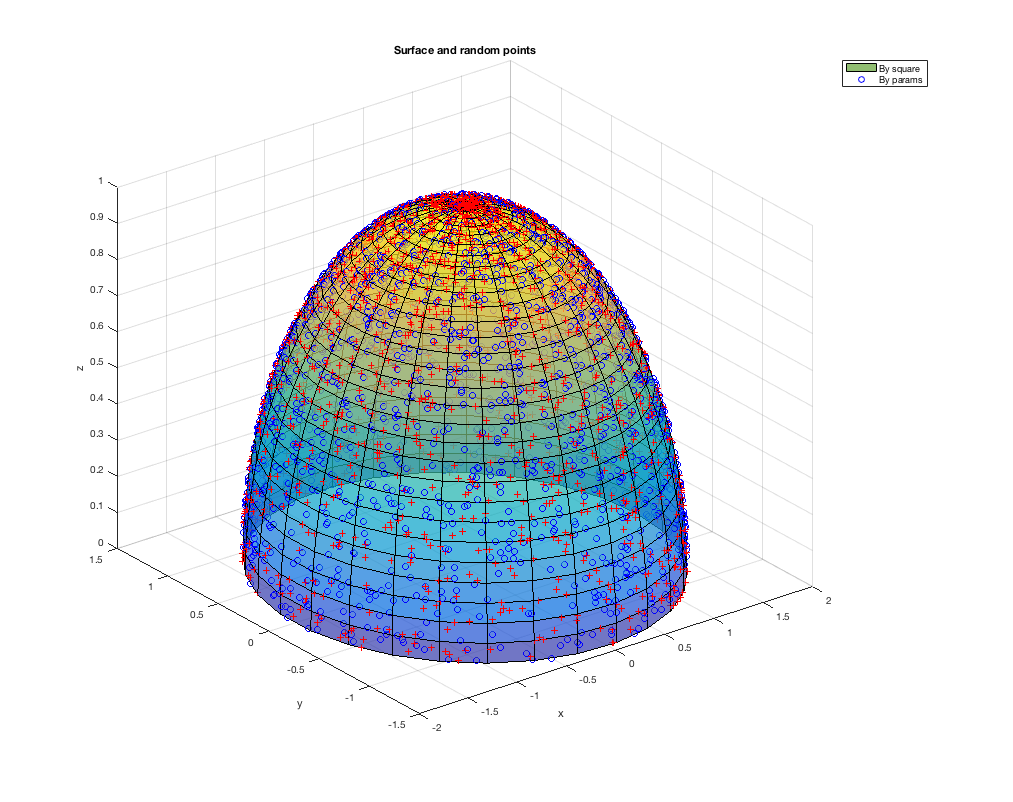
\includegraphics[width=\linewidth]{figure1.png}
\end{figure}
\end{document}

